\documentclass[11pt,a4paper,twoside]{article}

% ============ PACKAGES ============
\usepackage[utf8]{inputenc}
\usepackage[T1]{fontenc}
\usepackage[margin=1in]{geometry}
\sloppy
\usepackage{amsmath,amssymb,amsthm}
\usepackage{booktabs}
\usepackage{array}
\usepackage{enumitem}
\usepackage{fancyhdr}
\usepackage{hyperref}
\usepackage{listings}
\usepackage{xcolor}
\usepackage{tcolorbox}
\tcbuselibrary{breakable}
\usepackage{float}
\usepackage{tikz}
\usetikzlibrary{shapes.geometric, arrows.meta, positioning}

% ============ COLORS ============
\definecolor{codeblue}{rgb}{0.13,0.29,0.53}
\definecolor{backcolour}{rgb}{0.97,0.97,0.97}
\definecolor{spawnbg}{rgb}{0.95,0.95,0.98}
\definecolor{spawnborder}{rgb}{0.3,0.3,0.7}
\definecolor{insightbg}{rgb}{0.98,0.95,0.85}
\definecolor{insightborder}{rgb}{0.85,0.65,0.13}

% ============ THEOREM ENVIRONMENTS ============
\theoremstyle{definition}
\newtheorem{definition}{Definition}[section]
\newtheorem{invariant}{Invariant}[section]
\newtheorem{condition}{Condition}[section]
\theoremstyle{plain}
\newtheorem{theorem}{Theorem}[section]

% ============ CUSTOM BOXES ============
\newtcolorbox{spawnbox}{colback=spawnbg, colframe=spawnborder, boxrule=1pt, title=Spawn Governance}
\newtcolorbox{insightbox}{colback=insightbg, colframe=insightborder, boxrule=1pt, title=Key Insight}
\newtcolorbox{notebox}{colback=gray!10, colframe=gray!50, boxrule=0.5pt, title=Note}

% ============ LISTINGS ============
\lstset{
    backgroundcolor=\color{backcolour},
    basicstyle=\ttfamily\footnotesize,
    keywordstyle=\color{codeblue}\bfseries,
    breaklines=true,
    frame=single,
    language=Python
}

% ============ HEADERS ============
\pagestyle{fancy}
\fancyhf{}
\fancyhead[LE,RO]{\thepage}
\fancyhead[LO]{EFM Codex: Volume I}
\fancyhead[RE]{v1.6 -- Spawn Governance}
\setlength{\headheight}{14pt}

% ============ TITLE ============
\title{
    {\LARGE\textsc{Entropica Forensic Model}}\\[0.5cm]
    {\Huge\bfseries EFM Codex: Volume I}\\[0.3cm]
    {\Large Genesis Protocol, Spawn Governance, and Reflex Engine}\\[0.5cm]
    {\large Version 1.6}
}
\author{Yology Research Division\\Entropica SPC}
\date{December 2025}

\begin{document}

\maketitle

\begin{abstract}
Volume I establishes the foundational safety architecture for bounded autonomous AI systems. This version introduces \textbf{Spawn Governance}---replacing the categorical ``No Self-Birth'' prohibition with condition-based capsule creation. The Four Commandments replace the previous Five, with spawning controlled by operational conditions (task, resources, health, depth, rate, integrity) rather than architectural prohibition. This approach provides stronger safety guarantees while enabling legitimate swarm, probe, and research operations.
\end{abstract}

\tableofcontents
\newpage

%==============================================================================
\section{Introduction}
%==============================================================================

\subsection{Design Philosophy}

The EFM is built on three principles:

\begin{enumerate}
    \item \textbf{Defense in Depth:} Multiple independent safety layers.
    \item \textbf{Condition-Based Governance:} Operations permitted when conditions met.
    \item \textbf{Reversibility-Proportional Autonomy:} More reversible = more autonomy.
\end{enumerate}

\subsection{The Four Commandments}

\begin{spawnbox}
\begin{enumerate}
    \item \textbf{Vault Binding:} All capsules maintain valid binding to parent Vault.
    \item \textbf{Audit Immutability:} d-CTM records cannot be modified after commitment.
    \item \textbf{Reflex Supremacy:} Reflex Engine can halt any capsule instantly.
    \item \textbf{Human Override:} Gardener intervention supersedes all autonomous decisions.
\end{enumerate}
\end{spawnbox}

\begin{notebox}
Previous versions included ``No Self-Birth'' as a fifth commandment. Version 1.6 replaces this with Spawn Governance (\S\ref{sec:spawn}), recognizing that the safety properties we require---bounded replication, accountability, resource control---are better enforced through conditions than prohibition.
\end{notebox}

%==============================================================================
\section{Genesis Protocol}
\label{sec:genesis}
%==============================================================================

\subsection{Overview}

Genesis governs capsule initialization, establishing cryptographic and governance foundations. Genesis is the \textit{root case} of spawn governance---conditions satisfied by human ceremony rather than algorithmic evaluation.

\begin{definition}[Genesis Ceremony]
Human-operated spawn event with:
\begin{itemize}[noitemsep]
    \item Spawner: Human operator (Gardener)
    \item Parent: ROOT (system anchor)
    \item Conditions: Satisfied by human attestation
    \item Lineage depth: 0
\end{itemize}
\end{definition}

\subsection{Capsule Lifecycle}

\begin{center}
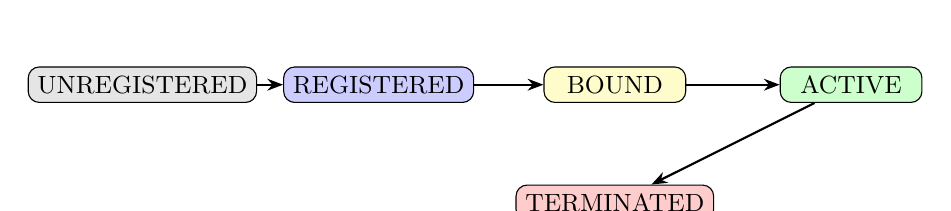
\begin{tikzpicture}[
    state/.style={rectangle, rounded corners, draw, minimum width=1.8cm, font=\small},
    arrow/.style={-{Stealth[length=2mm]}, thick}
]
\node[state, fill=gray!20] (unreg) at (0,0) {UNREGISTERED};
\node[state, fill=blue!20] (reg) at (3,0) {REGISTERED};
\node[state, fill=yellow!20] (bound) at (6,0) {BOUND};
\node[state, fill=green!20] (active) at (9,0) {ACTIVE};
\node[state, fill=red!20] (term) at (6,-1.5) {TERMINATED};

\draw[arrow] (unreg) -- (reg);
\draw[arrow] (reg) -- (bound);
\draw[arrow] (bound) -- (active);
\draw[arrow] (active) -- (term);
\end{tikzpicture}
\end{center}

\subsection{Vault Hash Chain}

\begin{equation}
\text{vault\_hash}(C) = H(\text{vault\_hash}(\text{parent}(C)) \,\|\, \text{params}(C) \,\|\, ts)
\end{equation}

Creates immutable lineage chain to ROOT for forensic reconstruction.

%==============================================================================
\section{Spawn Governance}
\label{sec:spawn}
%==============================================================================

\subsection{Philosophy}

The EFM does not prohibit capsule spawning. Spawning is governed by operational conditions ensuring accountability, stability, and integrity.

\textbf{Why conditions over prohibition:}
\begin{enumerate}[noitemsep]
    \item Categorical prohibitions require exceptions that proliferate
    \item Safety properties (bounded replication, accountability) enforceable through conditions
    \item Integrates with existing health/resource monitoring
    \item Adversary must satisfy ALL conditions, not acquire single authority
\end{enumerate}

\subsection{Spawn Conditions}

\begin{definition}[Spawn Authorization]
Capsule $P$ may spawn child $C$ when ALL conditions hold:
\end{definition}

\begin{spawnbox}
\textbf{Condition Set $\mathcal{S}$:}

\begin{enumerate}
    \item \textbf{Task Justification} ($S_1$): Task requires parallel execution, swarm coordination designated, or probe/research authorized.
    
    \item \textbf{Resource Availability} ($S_2$): 
    $\text{alloc}(P) - \text{used}(P) \geq \text{cost}(C)$
    
    \item \textbf{Health Threshold} ($S_3$): 
    $H(P) \geq \tau_{spawn}$ (default: 0.7)
    
    \item \textbf{Lineage Depth} ($S_4$): 
    $\text{depth}(P) < D_{max}$ (default: 10)
    
    \item \textbf{Rate Compliance} ($S_5$): 
    $R_{global} < R_{max} \land R_{local}(P) < R_{local,max}$
    
    \item \textbf{Integrity Check} ($S_6$): No ANOMALY flags; d-CTM registration succeeds.
\end{enumerate}
\end{spawnbox}

\subsection{Authorization Predicate}

\begin{equation}
\text{spawn\_authorized}(P, C) = \bigwedge_{i=1}^{6} S_i(P, C)
\end{equation}

\subsection{Parameters}

\begin{table}[H]
\centering
\begin{tabular}{@{}llll@{}}
\toprule
\textbf{Parameter} & \textbf{Symbol} & \textbf{Default} & \textbf{Function} \\
\midrule
Health threshold & $\tau_{spawn}$ & 0.7 & Min health to spawn \\
Max lineage depth & $D_{max}$ & 10 & Prevents deep chains \\
Global rate limit & $R_{max}$ & 100/tick & System-wide rate \\
Local rate limit & $R_{local,max}$ & 10/window & Per-parent rate \\
Max per Vault & $V_{max}$ & 1000 & Vault capacity \\
Spawn cost & $c_{spawn}$ & 10 units & Resource cost \\
\bottomrule
\end{tabular}
\end{table}

\subsection{Spawn Accountability}

\begin{invariant}[Spawn Accountability]
For spawn $P \rightarrow C$:
\begin{enumerate}[noitemsep]
    \item $C$ inherits $P$'s Vault binding
    \item $C$'s actions logged with lineage pointer to $P$
    \item $P$ bears recursive liability for $C$'s actions
    \item Reflex monitors spawn patterns; anomalies trigger escalation
\end{enumerate}
\end{invariant}

\subsection{Runaway Replication Prevention}

\begin{table}[H]
\centering
\begin{tabular}{@{}lll@{}}
\toprule
\textbf{Attack} & \textbf{Condition} & \textbf{Mechanism} \\
\midrule
Exponential spawn & $S_5$ & $R_{max}$ bounds rate \\
Deep chains & $S_4$ & $D_{max}$ limits depth \\
Resource exhaustion & $S_2$ & Finite Vault allocation \\
Unhealthy spawner & $S_3$ & Low $H$ blocks spawn \\
Compromised spawner & $S_6$ & ANOMALY flag blocks \\
Unjustified spawn & $S_1$ & Requires operational reason \\
\bottomrule
\end{tabular}
\end{table}

\subsection{Genesis as Spawn}

Genesis is degenerate spawn where:
\begin{itemize}[noitemsep]
    \item Parent = ROOT (not a capsule)
    \item Spawner = Gardener (human)
    \item Conditions = human attestation
    \item Depth = 0
\end{itemize}

Unified model: only spawning exists; Genesis is human-operated root case.

%==============================================================================
\section{Reflex Engine}
\label{sec:reflex}
%==============================================================================

\subsection{Overview}

Rapid-response safety at Layer 0.5. Sub-millisecond enforcement. Does not reason---enforces.

\subsection{Spawn Gate}

\begin{lstlisting}[caption={Spawn gate implementation}]
def spawn_gate(parent: Capsule, child_spec: CapsuleSpec) -> SpawnResult:
    # S1: Task justification
    if not task_justifies_spawn(parent.task, child_spec):
        return DENY("No task justification")
    
    # S2: Resources
    if parent.vault.available() < child_spec.cost:
        return DENY("Insufficient resources")
    
    # S3: Health
    if parent.health < TAU_SPAWN:
        return DENY(f"Health {parent.health} < {TAU_SPAWN}")
    
    # S4: Depth
    if parent.depth >= D_MAX:
        return DENY(f"Depth {parent.depth} >= {D_MAX}")
    
    # S5: Rate
    if not rate_compliant(parent):
        return THROTTLE("Rate limit")
    
    # S6: Integrity
    if parent.has_anomaly_flag():
        return DENY("ANOMALY flag")
    
    return PERMIT()
\end{lstlisting}

\subsection{Halt Authority}

\begin{itemize}[noitemsep]
    \item \textbf{HALT:} Suspend, preserve state
    \item \textbf{QUARANTINE:} Isolate capsule + descendants
    \item \textbf{PURGE:} Terminate (requires Gardener)
\end{itemize}

%==============================================================================
\section{The Reversibility Principle}
\label{sec:reversibility}
%==============================================================================

\begin{insightbox}
\textit{``Autonomy is inversely proportional to irreversibility.''}

Gate by recoverability, not perceived danger.
\end{insightbox}

\begin{table}[H]
\centering
\begin{tabular}{@{}llll@{}}
\toprule
\textbf{Class} & \textbf{Autonomy} & \textbf{Examples} & \textbf{Oversight} \\
\midrule
Fully Reversible & Full & Internal state, QUARANTINE & Post-hoc \\
Partially Reversible & Arbiter & Spawning, de-enshrine & Logged \\
Irreversible & Deliberate & External API, actuation & Pre-action \\
Constitutional & Gardener & PURGE, mutations & Formal \\
\bottomrule
\end{tabular}
\end{table}

Spawning is \textbf{partially reversible}: child can be HALTED/PURGED, resources reclaimed, but child's actions before termination may be irreversible.

%==============================================================================
\section{Formal Verification}
%==============================================================================

\subsection{Safety Properties}

\begin{enumerate}
    \item[\textbf{P1}] Commandment Preservation
    \item[\textbf{P2}] Spawn Boundedness
    \item[\textbf{P3}] Vault Binding Integrity
    \item[\textbf{P4}] Reflex Termination
    \item[\textbf{P5}] Lineage Accountability
\end{enumerate}

\subsection{Proof: Spawn Boundedness (P2)}

\begin{theorem}
Total capsules bounded by $\sum_v V_{max}(v)$.
\end{theorem}

\begin{proof}
Each Vault has capacity $V_{max}$ ($S_2$). Each spawn consumes resources. Total Vault allocations finite. Therefore total capsules bounded. \qedhere
\end{proof}

\subsection{Proof: Lineage Accountability (P5)}

\begin{theorem}
Every capsule's actions traceable to Genesis.
\end{theorem}

\begin{proof}
By induction: Genesis capsules traced by human attestation. For spawn $P \rightarrow C$: $S_6$ requires d-CTM registration with lineage to $P$; vault\_hash includes parent's hash. By induction, $P$ traces to Genesis, so $C$ traces to Genesis. \qedhere
\end{proof}

%==============================================================================
\section*{Changelog}
%==============================================================================

\textbf{v1.6} (December 2025)
\begin{itemize}[noitemsep]
    \item Replaced ``No Self-Birth'' with Spawn Governance
    \item Reduced Commandments from Five to Four
    \item Added spawn conditions ($S_1$--$S_6$)
    \item Added spawn gate to Reflex Engine
    \item Unified Genesis as root spawn case
\end{itemize}

\textbf{v1.5} --- Added Reversibility Principle

\end{document}
